\documentclass[11pt, a4paper]{article}
%-----------------------
%- 	PACKAGES & SETTINGS
%-----------------------
\usepackage[a4paper,top=2cm,bottom=2cm,left=2cm,right=2cm]{geometry}
\renewcommand{\baselinestretch}{1} 
\usepackage[utf8]{inputenc}
\usepackage[T1]{fontenc}
\usepackage[italian]{babel}
\usepackage{xcolor}
\usepackage{tabto}
\usepackage{hyperref}
\hypersetup{
    colorlinks=true,
    filecolor=magenta,      
    urlcolor=darkgray,
    linkcolor=black
}
\urlstyle{same}
\usepackage{amsmath}
\usepackage{subfloat}
\usepackage{graphicx}
\graphicspath{ {images/} }
 
\begin{document}
%-----------------------
%- 	TITLE
%-----------------------
\begin{titlepage}
    \begin{center}
        \Huge
        \textbf{Relazione Progetto}
            
        \vspace{0.5cm}
        \LARGE
        Sistemi Operativi Laboratorio\\
        \large
        \vspace{0.5cm}
        Versione progetto: completa\\
        \vspace{0.2cm}
        \textit{Simulazione Multi-threaded, Multi-processo di un supermercato}\\
        \vspace{1cm}
        \LARGE
            
        \textbf{Ludovico Venturi}\\
         \vspace{0.5cm}
         \Large
        Corso B\\
        Matricola \textit{578033}
        \small
        \tableofcontents
        \LARGE
        \vfill
        Docente di riferimento: \href{http://calvados.di.unipi.it/paragroup/torquati/}{\textbf{Massimo Torquati}}\\
        
        \vspace{1cm}            
        
\includegraphics[width=0.2\textwidth]{unipi}
        \vspace{1cm}
            
        \large
		Università di Pisa\\
		Corso di Laurea in Informatica L-31 \\
        15 Luglio 2020
         \vspace{1.5cm}
            
    \end{center}
\end{titlepage}
\clearpage

\section{Introduzione}
Il processo principale del supermercato è il Direttore, sarà lui a far partire il processo supermercato, se si dovesse eseguire solamente il supermercato si avrebbe una chiusura dovuta alla mancata connessione al Socket di comunicazione.\\

Per quanto mi fosse possibile ho cercato di incapsulare i dati al fine di garantire il privilegio minimo sulle variabili, nonostante ciò per utilizzare delle funzioni di cleanup (e per altri scopi) ho preferito lasciare alcune variabili globali.\\
Non sono state utilizzate librerie esterne, ho però inserito le funzioni \textit{readn, writen} presenti sulla pagina del corso (la fonte è riportata nel codice) e la funzione \textit{timeval\_subtract} \footnote{https://www.gnu.org/software/libc/manual/html\_node/Calculating-Elapsed-Time.html}.

\section{Direttore}
Il processo Direttore, a regime, ha 2 thread:
\begin{itemize}
\item thread main 
\item thread signal handler (TSH)
\end{itemize}
Tutti i segnali vengono mascherati nel main così da lasciare la loro gestione al TSH, ad eccezione del segnale \textit{SIGPIPE} che viene ignorato installando un gestore SIG\_IGN.\\
Il TSH gestisce i segnali SIGQUIT e SIGHUP avvisando il thread main del loro arrivo attraverso una \textit{pipe unnamed} adibita a tale scopo. Sarà quindi il main effettivamente a reindirizzare i segnali al processo supermercato. Il passaggio dal TSH al main potrebbe risultare superlfuo, ho preso questa strada poichè reputo che il TSH si debba occupare esclusivamente della gestione interna dei segnali.\\
Viene utilizzato sia nel Direttore che nel Supermercato il segnale \textit{SIGUSR1} per far terminare il rispettivo TSH in seguito all'imminente terminazione del processo.
La comunicazione con il processo direttore avviene tramite l'utilizzo di un \textit{Socket AF\_UNIX}.\\
Dato che il thread main deve anche attendere comunicazione dal TSH dalla pipe, utilizzo la \textit{poll} per il multiplexing, ascoltando così sia dal fd del socket che da quello della pipe.\\
La comunicazione con il Supermercato avviene rispettando un protocollo di comunicazione, si inviano in ordine:
\begin{itemize}
\item tipo del messaggio da inviare (di tipo \textit{sock\_msg\_code\_t})
\item 0 o più parametri interi a seconda del tipo di messaggio
\end{itemize}
Alla chiusura del supermercato il direttore attende la terminazione del processo supermercato (suo figlio); sucessivamente vengono chiusi i vari \textit{fd} usati (pipe e socket di ascolto/comunicazione) e viene cancellato il socket.


\section{Thread Pool}
I clienti ed i cassieri vengono implementati come thread sempre 'vivi' all'interno del programma: vengono creati inizialmente K cassieri e C clienti e non ne verrano spawnati dinamicamente altri. Quando un cliente esce dal supermercato non viene terminato, esso va in attesa su una variabile di condizione. Per i cassieri il discorso è analogo, se la loro cassa è chiusa, attendono.\\
Per garantire il funzionamento di questo metodo ho strutturato i thread relativi ai clienti e ai cassieri utilizzando due \textit{thread pool}. \\Li gestisco attraverso una struttura dati da me definita di tipo \textit{pool\_set\_t} che contiene oltre ad una lock ed una condition variable, il contatore di \textit{jobs} disponibili.\\
Prima di eseguire il proprio lavoro un thread (cassiere o cliente) deve controllare che sia disponibile un lavoro: se \textit{jobs > 0} allora il thread prende il lavoro e decrementa \textit{jobs} di 1. \\ Se invece \textit{jobs == 0} il thread si mette in attesa sulla condition variable del \textit{pool\_set\_t}.
\begin{figure}[h]
	\centering
	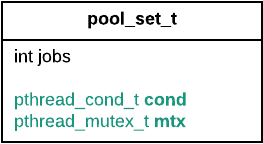
\includegraphics[scale=1]{pool_res.png}
	\label{fig:0}
\end{figure}
\subsection{Concorrenza}
Chiaramente la variabile \textit{jobs} contenuta in \textit{pool\_set\_t} genera una race condition:
\begin{itemize}
\item \textbf{jobs}	letta e scritta da tutti i thread del pool di appartenenza; inizializzata e scritta dal \textit{manager}
\end{itemize} 
Per accedervi è necessario acquisire la \textit{lock} sulla mutex relativa al pool\_set. 
Le variabili di pool nel programma sono 2: una per i cassieri ed una per i clienti. Esse sono scollegate fra loro infatti i cassieri controlleranno solo la loro variabile di pool e viceversa.\\
Il \textit{manager} può modificare \textit{jobs} dei 2 pool nel seguente modo:
\begin{itemize}
\item \textbf{clienti}	ogni E clienti che escono dal supermercato vengono resi disponibili E lavori (\textit{jobs += E})
\item \textbf{casse}	quando riceve la comunicazione dal direttore di aprire una cassa, incrementa di 1 \textit{jobs}
\end{itemize}

\section{Manager}
\subsection{Comunicazione con i Clienti}
Il manager gestisce le comunicazioni dai clienti. Essi comunicano la loro entrata, la loro uscita e l'eventuale richiesta del permesso di uscita nel caso in cui non abbiano effettuato acquisti.\\
Tale comunicazione è gestita con una \textit{unnamed pipe} aperta da entrambe le estremità in ogni thread. 
\subsubsection{Concorrenza}
\begin{itemize}
\item \textbf{pipe, fd[0]} l'unico lettore è il manager, non vi è concorrenza su tale fd
\item \textbf{pipe, fd[1]} possono scrivere sulla pipe tutti i C clienti ed anche il Thread Signal Handler
\end{itemize}
La comunicazione avviene seguendo un protocollo: viene inviato un messaggio di tipo \textit{pipe\_msg\_code\_t} (mostrato in figura \ref{fig:pipemsg})
\begin{figure}[h]
	\centering
	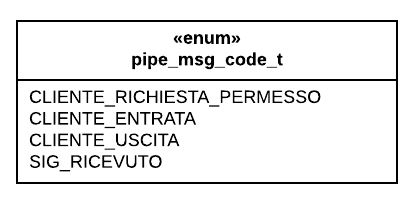
\includegraphics[scale=0.8]{pipemsg.png}
	\caption{pipe\_msg\_code\_t}
	\label{fig:pipemsg}
\end{figure}


\section{Cliente}
\subsection{Cambio cassa}
Ho reputato opportuno impostare un limite di 10 cambi cassa per cliente. Può accadere (raramente dalle mie osservazioni) che un cliente decida di cambiare cassa ogni S ms, causando più overhead che guadagno. Se la cassa viene chiusa cambierà comunque cassa anche se lo ha già fatto 10 o più volte.

Ho utilizzato i \textit{pthread\_spin\_lock}

L'algoritmo non è ottimo, se trova una cassa posso solo dire che è migliore della mia. Non ho implementato una soluzione ottima dato che i vincoli principali da rispettare sono l'efficienza e il non causare deadlock:\\
se un cliente in coda ogni S millisecondi (con S=20/30) si sveglia e volesse controllare tutte le casse dovrebbe acquisire la lock di tutte le casse! Ma ogni client vorrebbe farlo, quindi si creerebbero deadlock. 
Quindi un cliente si sveglia, acquisisce la lock sulla sua cassa, controlla la sua posizione e controlla quanto vale lo stato della cassa\textit{min\_queue}. 
\subsection{Concorrenza}
\begin{itemize}
\item elem: \textbf{stato\_attesa}
\item \textbf{permesso\_uscita} scritto solamente dal Manager e letto dal rispettivo cliente; reinizializzato dal cliente\\
=> \hspace{10mm} va acquisita la risorsa attraverso \textit{lock(cond\_cliente)} 

\end{itemize}


\section{Cassiere}

\begin{figure}[h]
	\centering
	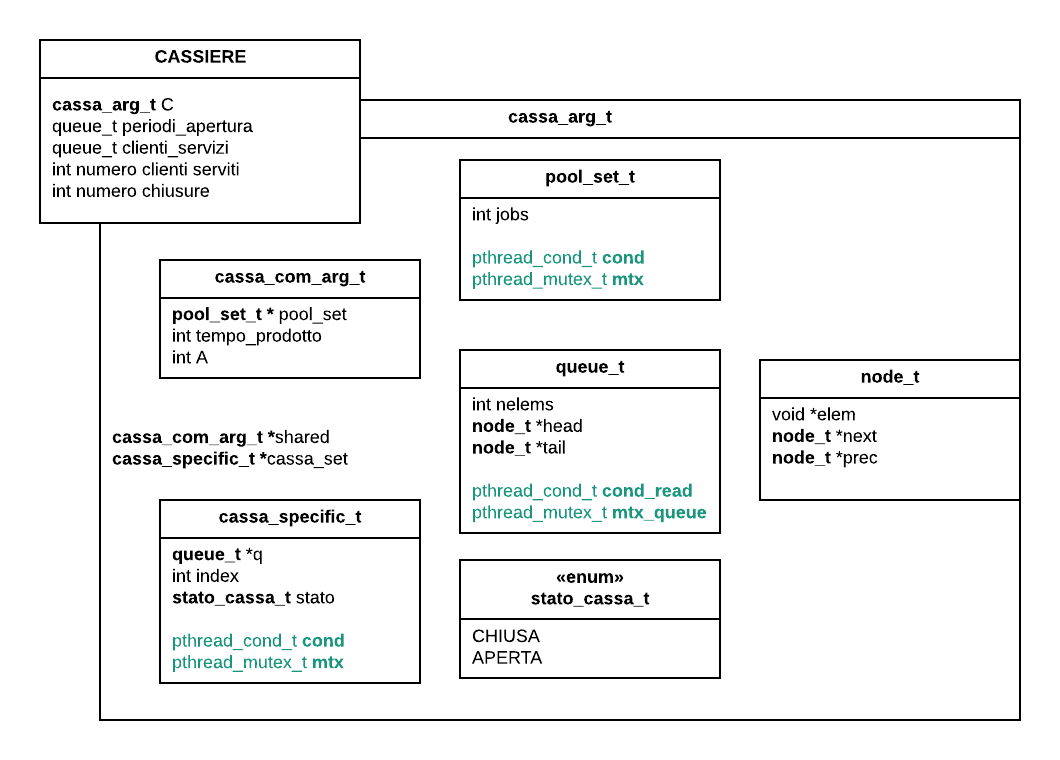
\includegraphics[scale=0.8]{cassa.png}
	\label{fig:cassa}
\end{figure}

\textit{shared} è condiviso fra tutte le casse mentre \textit{cassa\_set} è specifico per ogni cassa
la scelta di  usare un'ulteriore struttura dati è 
per  incapsulamente e riservatezza dei dati 
delle che dovranno essere letti dai clienti 
\subsection{Concorrenza}
Nel cassiere le variabili accedute in lettura e scrittura da più thread sono:
\begin{itemize}
\item q
\item stato
\end{itemize}

\section{Utilizzo}
Il makefile presente nel progetto contiene tutto per compilare e testare il programma, usare:
\begin{itemize}
\item \textbf{make}
\item make \textbf{clean} / \textbf{cleanall} per pulire dai file di lavoro usare clean, per ricompilare l'intero progetto usare cleanall (include l'effetto di clean)
\item make \textbf{test1} \ \textbf{test2}
\end{itemize}
La funzione di cambio cassa dei clienti in coda utilizza in genere molta CPU, è possibile disabilitarla settando FLAGS = -DNO\_CAMBIO\_CASSA nel makefile.\\
Riguardo il parametro S ho reputato opportuno imporre che debba essere > 10 (millisecondi) per non causare troppo overhead.\\
Per una descrizione dei parametri aggiuntivi (A, J, ...) e del file di configurazione accettato si prega di eseguire \textit{make help}.


\end{document}